%
% 2_beispiel.tex -- Wellengleichung tatsächlich lösen mit der Methode
%
% (c) 2025 Roman Cvijanovic & Nicola Dall'Acqua, Hochschule Rapperswil
%
% !TEX root = ../../buch.tex
% !TEX encoding = UTF-8
%

\section{Rechenbeispiele}\label{neuronal:section:rechenbeispiel}
\kopfrechts{Rechenbeispiele}

In diesem Abschnitt wird die zuvor vorgestellte Methode auf die Wellengleichung in zwei Dimensionen und die Burgers-Gleichung in einer Dimension angewendet.
Der Ablauf orientiert sich an den Schritten aus Abschnitt \ref{neuronal:section:herleitung}:
\begin{enumerate}
    \item Definition eines neuronalen Netzwerks
    \item Diskretisierung der Definitionsbereiche
    \item Aufbau der Funktion $L(\vartheta)$
    \item Minimierung von $L(\vartheta)$
    \item Qualitätsbewertung anhand von $L(\vartheta)$ und $L^1(\vartheta)$
\end{enumerate}

Sämtliche Resultate können mit dem Code im GitHub Repository \cite{neuronal:github_source_code} reproduziert werden.
Im Repository ist zusätzlich eine Readme-Datei abgelegt, welche einige Punkte bezüglich Reproduzierbarkeit klärt.

\subsection{Wellengleichung in zwei Dimensionen}\label{neuronal:subsection:wellengleichung}
\kopfrechts{Wellengleichung}
Die zu lösende Gleichung lautet
\begin{equation}
    \frac{\partial^2 u}{\partial t^2} = c^2 \left( \frac{\partial^2 u}{\partial x^2} + \frac{\partial^2 u}{\partial y^2} \right).
    \label{neuronal:wellengleichung}
\end{equation}
Die Konstante \( c \) ist die Ausbreitungsgeschwindigkeit der Welle. Der Einfachheit halber wird \( c = 1 \) festgelegt.
Zusätzlich werden die folgenden Anfangsbedingungen
\begin{equation}
    \begin{aligned}
        u(x, y, 0) &= \sin(\pi x) \sin(\pi y)\\
        \frac{\partial u(x, y, 0)}{\partial t} &= 0
    \end{aligned}
    \label{neuronal:wellen_anfangs}
\end{equation}
sowie die Randbedingungen
\begin{equation}
    \begin{aligned}
        u(-2, y, t) &= 0\\
        u(2, y, t) &= 0\\
        u(x, -2, t) &= 0\\
        u(x, 2, t) &= 0
    \end{aligned}
    \label{neuronal:wellen_rand}
\end{equation}
verwendet.
Die Bereiche sind \( x, y \in [-2,2] \) und \( t \in [0,2] \).
Dieses Gleichungssystem hat eine analytische Lösung welche
\begin{equation}
    u(x, y, t) = \cos(c \pi \sqrt{2}\: t)\sin(\pi x)\sin(\pi y)
    \label{neuronal:wellen_analytisch}
\end{equation}
lautet.
Somit kann das neuronale Netzwerk zur Qualitätsbewertung direkt damit verglichen werden.

Das neuronale Netzwerk zur Lösung der Wellengleichung weicht leicht von der allgemeinen Definition im Abschnitt \ref{neuronal:subsection:struktur_nn} ab.
Zusätzlich zu den drei Variablen $x, y$ und $t$ wird dem Netzwerk der Wert der ersten Anfangsbedingung \eqref{neuronal:wellen_anfangs} als Input gegeben.
Somit ist das neuronale Netzwerk
\begin{align*}
    \hat{u}(x,\; y,\; t,\; u(x, y, 0);\; \vartheta),
\end{align*}
wobei
\begin{align*}
    u(x, y, 0) = \sin(\pi x) \sin(\pi y).
\end{align*}
Die Idee dabei ist, dass diese Anfangsbedingung auf eine bestimmte Art in der gesuchten Funktion $u$ vorkommen muss.
Daher ist es naheliegend, diese Anfangsbedingung als zusätzlichen Input zu verwenden.
Der konkrete Aufbau des neuronalen Netzwerks ist somit wie folgt:
\begin{itemize}
    \item 4 Teilfunktionen
    \item \( f_1 \): \( \mathbb{R}^4 \longrightarrow \mathbb{R}^{128} \) 
    \item \( f_{4} \): \( \mathbb{R}^{128} \longrightarrow \mathbb{R} \)
    \item Alle anderen Teilfunktionen: \( \mathbb{R}^{128} \longrightarrow \mathbb{R}^{128} \)
    \item Als Aktivierungsfunktion wird der hyperbolische Tangens verwendet
\end{itemize}
Das Netzwerk verfügt somit über 33'793 Parameter.
In der letzten Teilfunktion \( f_{4} \) wird keine Aktivierungsfunktion verwendet.
Grund dafür ist, dass der hyperbolische Tangens den Wertebereich \((-1, 1)\) hat, das Netzwerk aber zur Approximation der Wellengleichung den Wertebereich \( \mathbb{R} \) haben soll.

Wie im Abschnitt \ref{neuronal:subsection:diskretierung} beschrieben, werden insgesamt drei Datensätze verwendet.
Alle drei Datensätze bestehen aus je 50'000 Datenpunkten.
Weiter wurde je ein Fünftel der Datenpunkte für die Funktion \( L^1(\vartheta) \) abgetrennt und nicht im Optimierungsalgorithmus verwendet (siehe Abschnitt \ref{neuronal:subsection:qualitätsbewertung}).

Beendet man den Optimierungsalgorithmus nach 1500 Iterationen, findet sich eine gute Lösung.
Die Werte von $L(\vartheta)$ und $L^1(\vartheta)$ sind 4.011 bzw. 0.878 (siehe Abbildung \ref{fig:fehler_wave_good}), was zunächst nicht besonders vielversprechend ist.
Zusätzliche Iterationen des Optimierungsalgorithmus reduzieren zwar den Wert von $L(\vartheta)$ weiter, doch der Wert von $L^1(\vartheta)$ beginnt wieder anzusteigen.
Dies ist ein klassisches Phänomen im Gebiet des maschinellen Lernens und wird als \emph{Overfitting} bezeichnet.
\emph{Overfitting} bedeutet, dass das neuronale Netzwerk die Datenpunkte $F_t\cup A_t \cup B_t$, mit denen $L(\vartheta)$ berechnet wird, ``auswendig'' lernt.
Als Resultat versagt das Netzwerk bei den Datenpunkten $F_k\cup A_k \cup B_k$, mit denen $L^1(\vartheta)$ berechnet wird.
Daher wurde der Optimierungsalgorithmus nach 1500 Iterationen beendet, obwohl die Approximationsfehler nicht sehr tief sind.
\begin{figure}
    \centering
    \hspace*{-0.1\textwidth}
    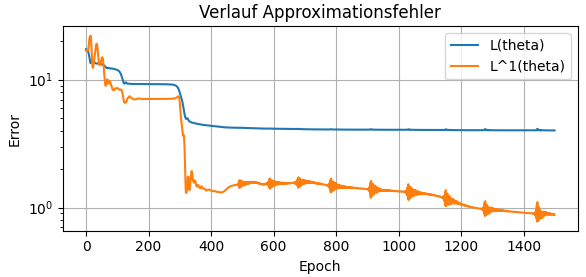
\includegraphics[width=0.7\textwidth]{papers/neuronal/images/approximation_error_wave_good.png}
    \caption{Verlauf des Approximationsfehlers der Wellengleichung während des Trainings}
    \label{fig:fehler_wave_good}
\end{figure}

Berechnet man nun die durchschnittliche Differenz des neuronalen Netzwerks und der analytischen Lösung \eqref{neuronal:wellen_analytisch}, erhält man 0.079.
Dieser Wert ist deutlich besser und deutet darauf hin, dass das neuronale Netzwerk eine gute Approximation liefert. 
Der Verlauf dieser Differenz ist in \ref{fig:differenz_wellen} dargestellt.
\begin{figure}
    \centering
    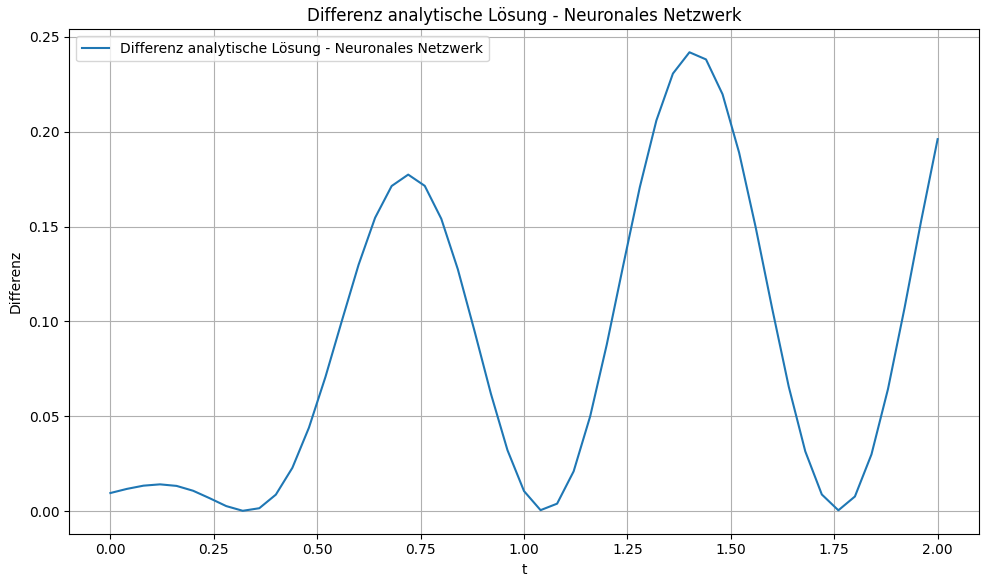
\includegraphics[width=0.7\textwidth]{papers/neuronal/images/wellen_analytisch_neuronal.png}
    \caption{Verlauf der Differenz Wellengleichung: Analytische Lösung - Neuronales Netzwerk}
    \label{fig:differenz_wellen}
\end{figure}

Der Lösungsplot ist in den Abbildungen \ref{fig:wellen_t0}, \ref{fig:wellen_t04}, \ref{fig:wellen_t136}, \ref{fig:wellen_t164} dargestellt.
In diesen Abbildungen ist auf der linken Seite das neuronale Netzwerk und auf der rechten Seite die analytische Lösung abgebildet.
Die Farben stellen die Wellenhöhen dar, rot bedeutet einen Wellenberg und blau ein Wellental.
Was in diesen Abbildungen deutlich zu sehen ist, ist dass das Netzwerk bei Übergängen von Wellenbergen zu Wellentälern (z.B. von \ref{fig:wellen_t0} zu \ref{fig:wellen_t04}) Fehler macht.
Dies wird deutlich wenn man $y$ bei $0.5$ fixiert und Lösungsplots für verschiedene $t$ erstellt (siehe Abbildung \ref{fig:loesung_wellen_fix_yt}).
In dieser Abbildungsreihe ist klar zu erkennen, dass diese Übergänge zwar stattfinden, aber chaotisch ablaufen.
Abgesehen davon sieht die Approximation visuell gut aus.
Die Approximation ist als Animation über den gesamten Zeitraum $t \in [0, 2]$ im GitHub Repository des Seminars \cite{neuronal:github_source_code}, im Unterverzeichnis \emph{wave\_equation} zu finden.
\begin{figure}
    \centering
    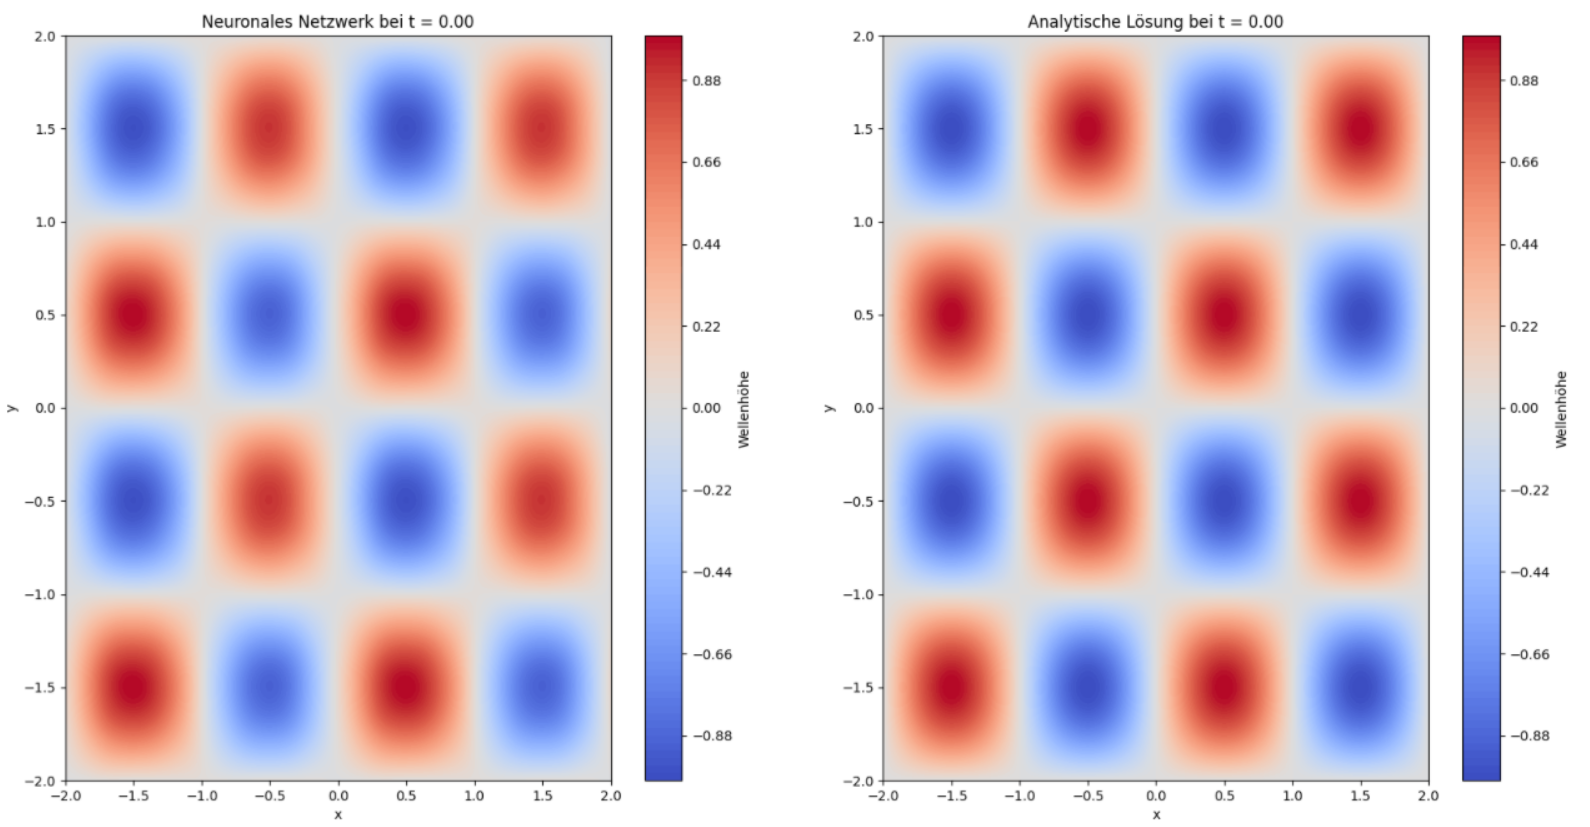
\includegraphics[width=\textwidth]{papers/neuronal/images/prediction_wave_t0.png}
    \caption{Wellengleichung $t = 0$}
    \label{fig:wellen_t0}
\end{figure}
\begin{figure}
    \centering
    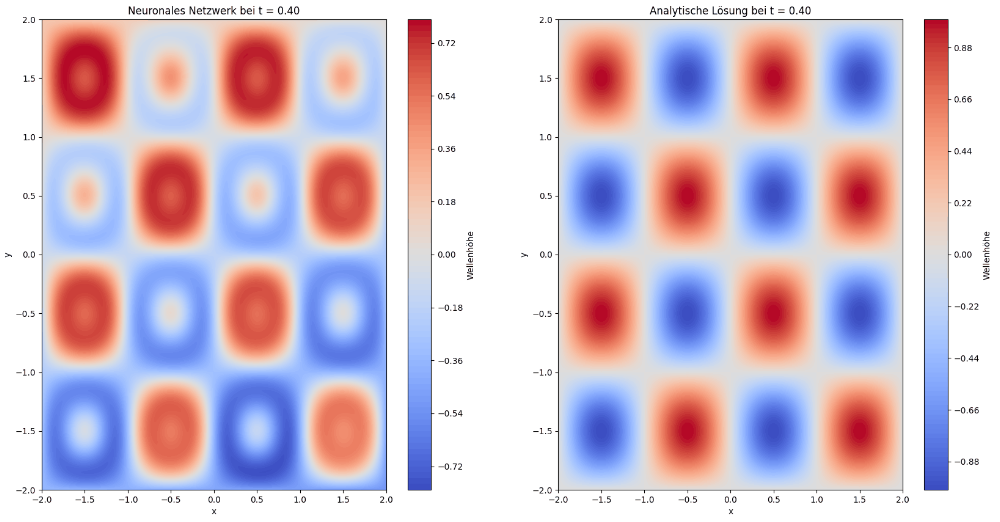
\includegraphics[width=\textwidth]{papers/neuronal/images/prediction_wave_t04.png}
    \caption{Wellengleichung $t = 0.4$}
    \label{fig:wellen_t04}
\end{figure}
\begin{figure}
    \centering
    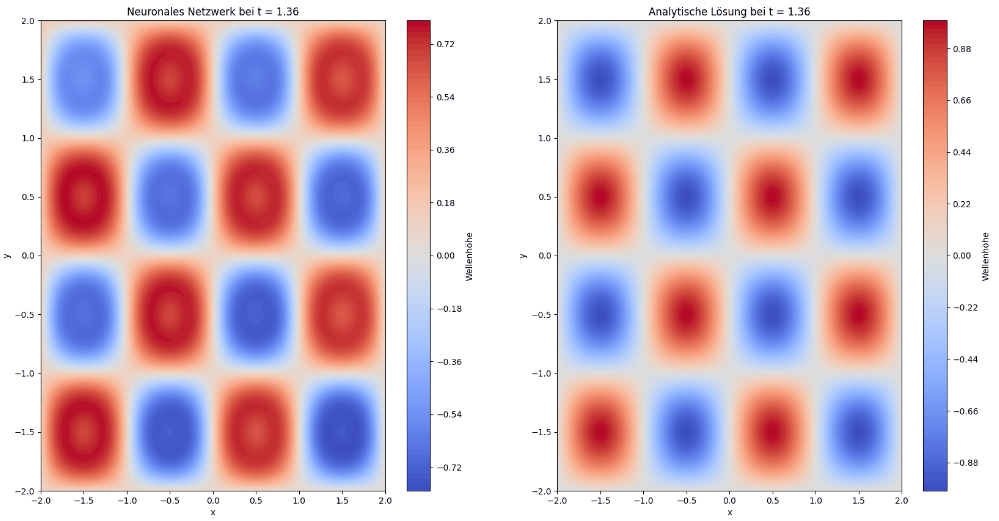
\includegraphics[width=\textwidth]{papers/neuronal/images/prediction_wave_t136.png}
    \caption{Wellengleichung $t = 1.36$}
    \label{fig:wellen_t136}
\end{figure}
\begin{figure}
    \centering
    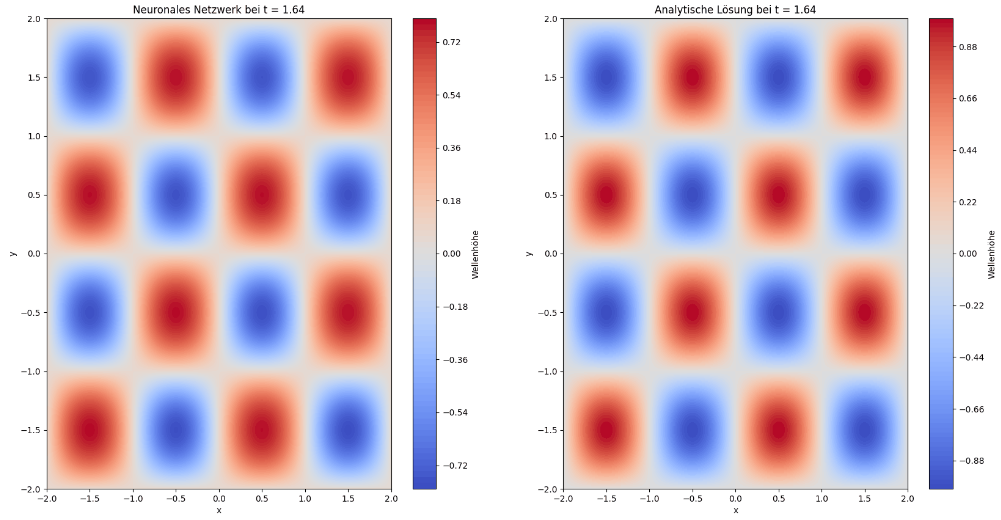
\includegraphics[width=\textwidth]{papers/neuronal/images/prediction_wave_t164.png}
    \caption{Wellengleichung $t = 1.64$}
    \label{fig:wellen_t164}
\end{figure}

\begin{figure}
    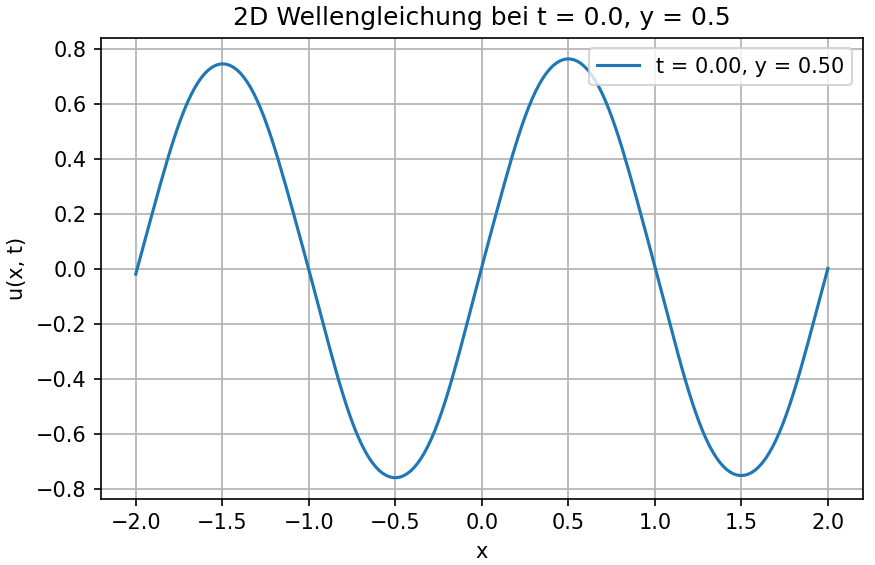
\includegraphics[width=0.48\textwidth]{papers/neuronal/images/wave_solution_t0.png}\hfill
    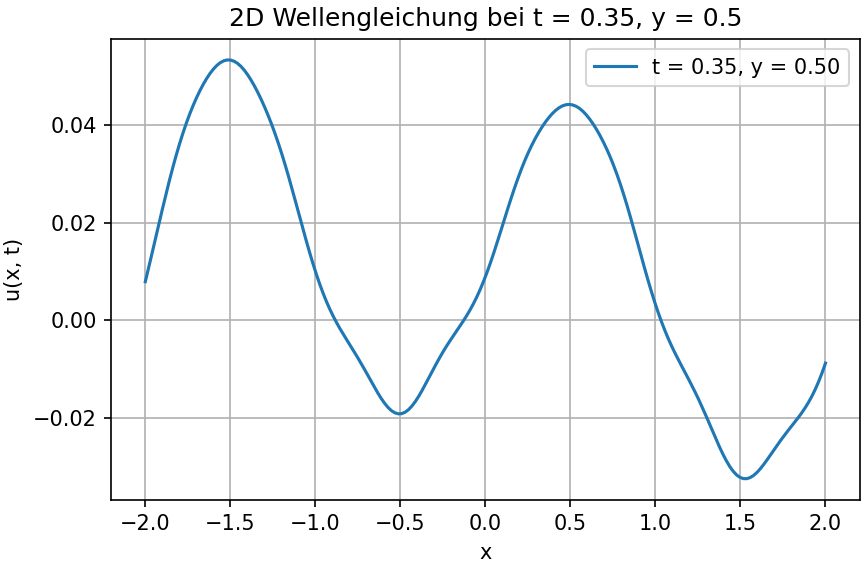
\includegraphics[width=0.48\textwidth]{papers/neuronal/images/wave_solution_t035.png}
    \\[\smallskipamount]
    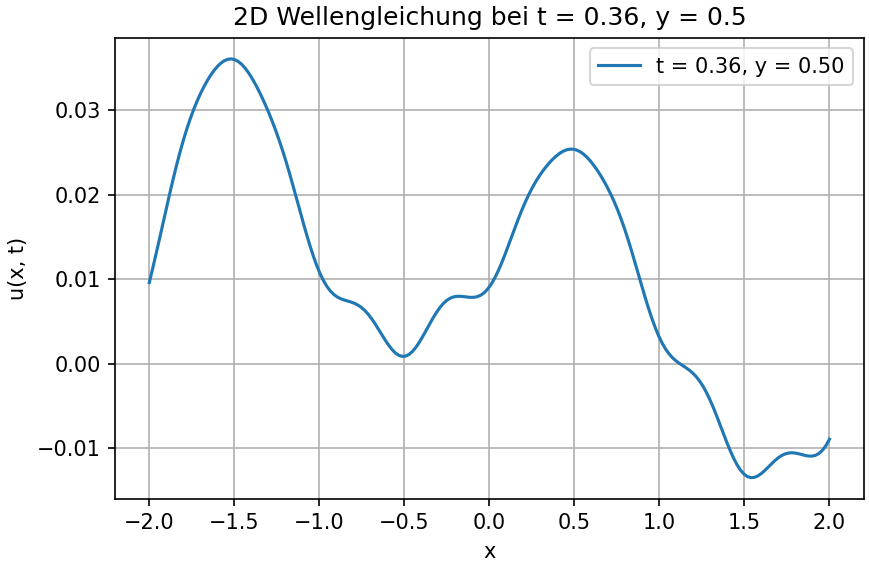
\includegraphics[width=0.48\textwidth]{papers/neuronal/images/wave_solution_t036.png}\hfill
    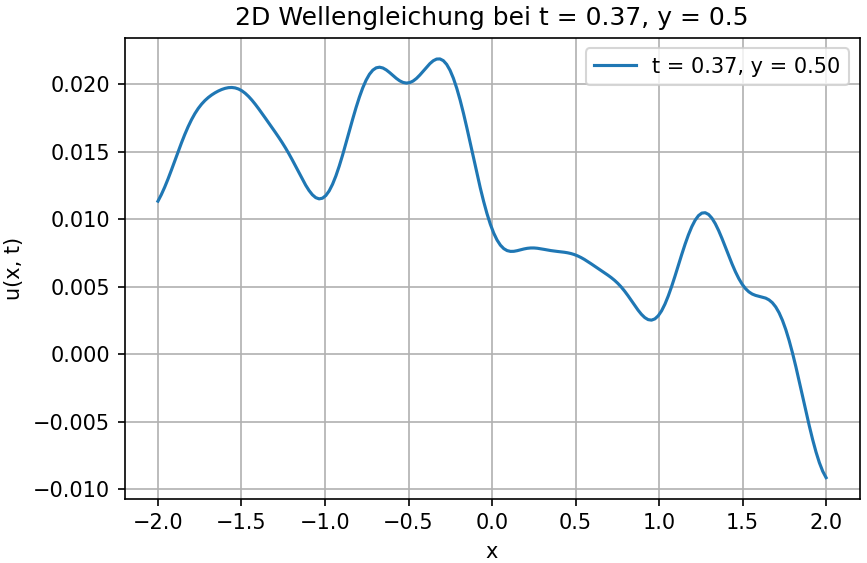
\includegraphics[width=0.48\textwidth]{papers/neuronal/images/wave_solution_t037.png}
    \\[\smallskipamount]
    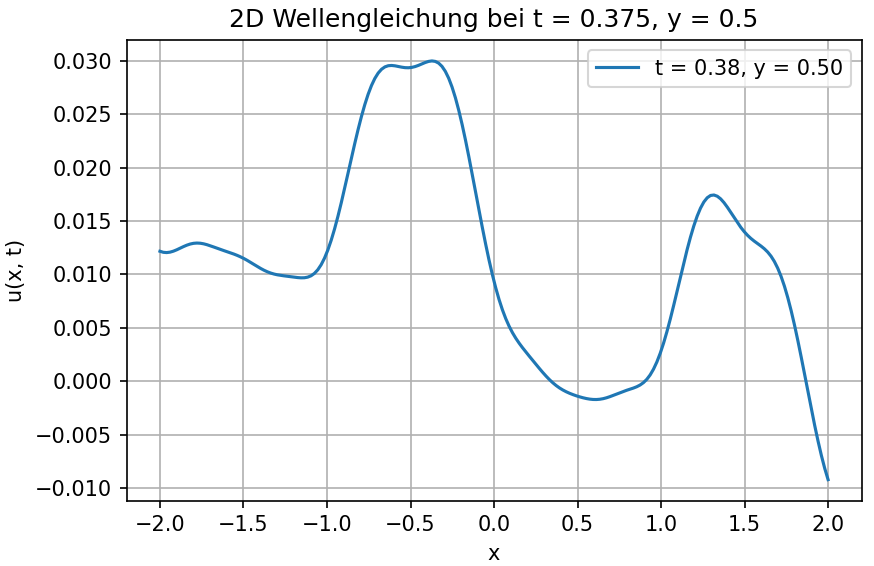
\includegraphics[width=0.48\textwidth]{papers/neuronal/images/wave_solution_t0375.png}\hfill
    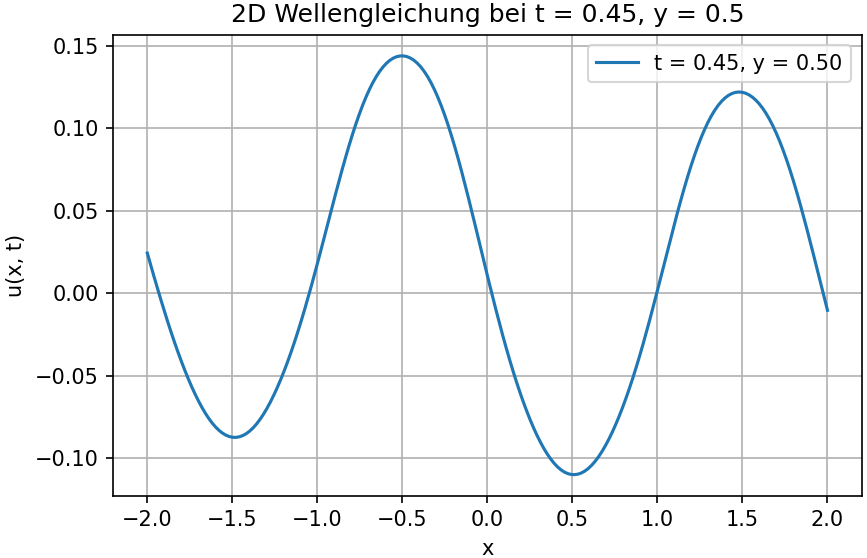
\includegraphics[width=0.48\textwidth]{papers/neuronal/images/wave_solution_t045.png}
    \caption{Lösungs-Plot der Wellengleichung zu verschiedenen Zeiten und $y = 0.5$}\label{fig:loesung_wellen_fix_yt}
\end{figure}

\subsection{Burgers-Gleichung}\label{neuronal:subsection:burgers_gleichung}
\kopfrechts{Burgers-Gleichung}
Die Burgers-Gleichung ist gegeben als
\begin{equation}
    \frac{\partial u}{\partial t} + u \frac{\partial u}{\partial x} = \nu \frac{\partial^2 u}{\partial x^2}.
    \label{neuronal:burgers}
\end{equation}
Der Diffusionskoeffizient \( \nu \) wird auf \( \nu = \frac{0.01}{\pi} \) festgelegt.
Die Anfangsbedingung
\begin{equation}
    u(0, x) = - \sin(\pi x)
    \label{neuronal:burgers_anfang}
\end{equation}
und die Randbedingung
\begin{equation}
    u(t, -1) = u(t, 1) = 0.
    \label{neuronal:burgers_rand}
\end{equation}
werden verwendet.
Die Bereiche sind \( x \in [-1,1] \) und \( t \in [0,1] \).

Das neuronale Netzwerk zur Lösung der Burgers-Gleichung ist folgendermassen aufgebaut:
\begin{itemize}
    \item 10 Teilfunktionen
    \item \( f_1 \): \( \mathbb{R}^2 \longrightarrow \mathbb{R}^{20} \) 
    \item \( f_{10} \): \( \mathbb{R}^{20} \longrightarrow \mathbb{R} \)
    \item Alle anderen Teilfunktionen: \( \mathbb{R}^{20} \longrightarrow \mathbb{R}^{20} \)
    \item Als Aktivierungsfunktion wird der hyperbolische Tangens verwendet
\end{itemize}
Das Netzwerk verfügt somit über 3441 Parameter.
In der letzten Teilfunktion \( f_{10} \) wird keine Aktivierungsfunktion verwendet.
Grund dafür ist, dass der hyperbolische Tangens den Wertebereich \((-1, 1)\) hat, das Netzwerk aber zur Approximation der Burgers-Gleichung den Wertebereich \( \mathbb{R} \) haben soll.

Wie im Abschnitt \ref{neuronal:subsection:diskretierung} beschrieben, werden insgesamt drei Datensätze verwendet.
Der Datensatz \( F \), in dem die Burgers-Gleichung gilt, besteht aus 5000 Datenpunkten.
Die Datensätze \( A \) und \( B \), in denen die Anfangsbedingungen bzw. die Randbedingungen gilten, bestehen jeweils aus 2000 Datenpunkten.
Weiter wurde je ein Fünftel der Datenpunkte für die Funktion \( L^1(\vartheta) \) abgetrennt und nicht im Optimierungsalgorithmus verwendet (siehe Abschnitt \ref{neuronal:subsection:qualitätsbewertung}).

Der Optimierungsalgorithmus \ref{neuronal:gradient_descent} durchlief 15'000 Iterationen, um geeignete Parameter für die Approximation zu finden.
Die Werte von \( L(\vartheta) \) und \( L^1(\vartheta) \) am Ende der Optimierung sind 0.003328 bzw. 0.003449.
Somit sind die mittleren Approximationsfehler des Netzwerks sehr gering.
Der Verlauf des Approximationsfehlers während der Optimierung ist in Abbildung \ref{fig:fehler_burgers} dargestellt.
\begin{figure}
    \centering
    \hspace*{-0.1\textwidth}
    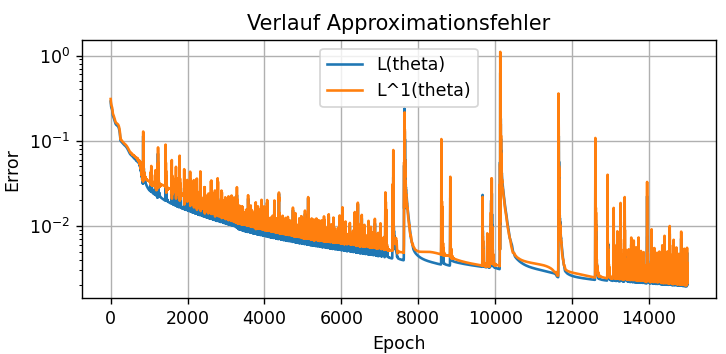
\includegraphics[width=0.7\textwidth]{papers/neuronal/images/approximation_error_burgers.png}
    \caption{Verlauf des Approximationsfehlers der Burgers-Gleichung während des Trainings}
    \label{fig:fehler_burgers}
\end{figure}

Wertet man das neuronale Netzwerk über die Bereiche von \( x \) und \( t \) aus, ergibt sich ein Plot der Lösung des neuronalen Netzwerks (siehe Abbildung \ref{fig:loesung_burgers}).
In dieser Abbildung laufen zwei sanfte Wellen aufeinander zu und kollidieren in einem scharfen Sprung.
\begin{figure}
    \centering
    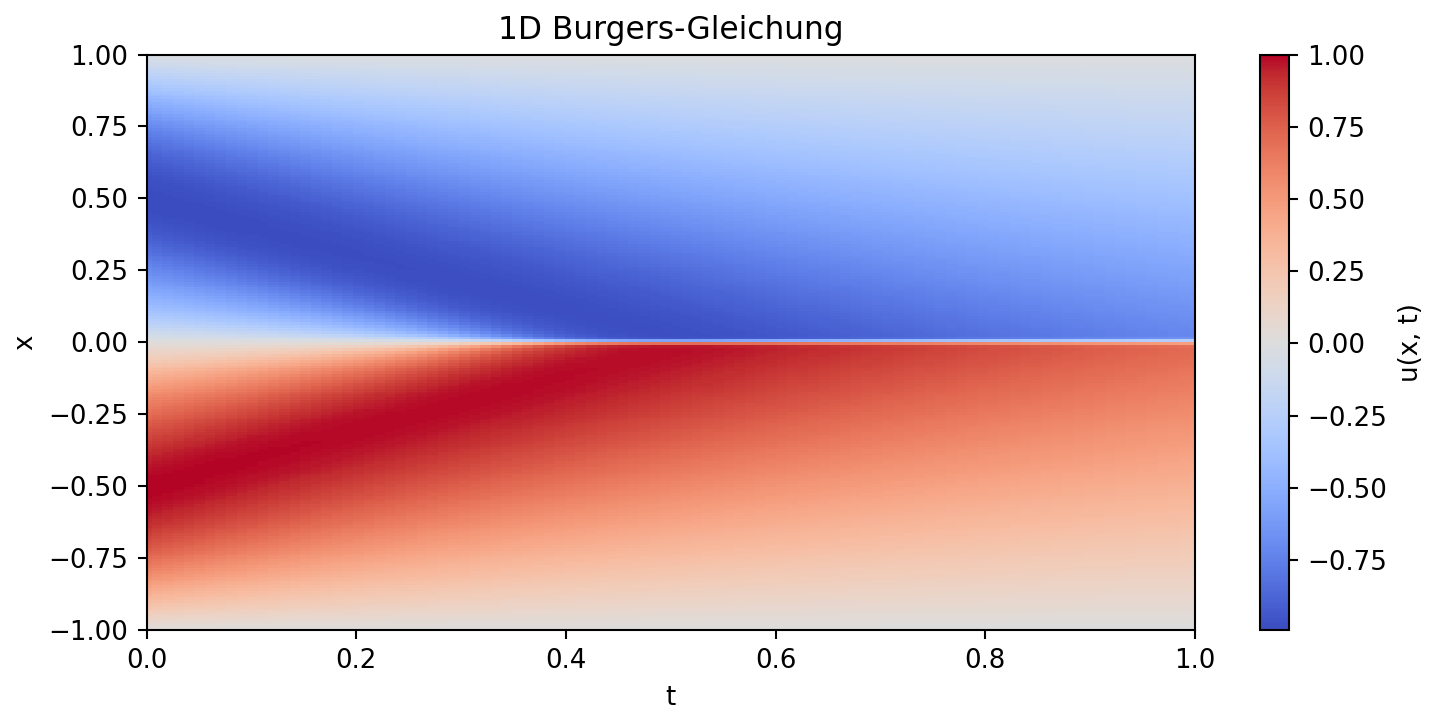
\includegraphics[width=0.8\textwidth]{papers/neuronal/images/prediction_burgers_net.png}
    \caption{Lösungs-Plot der Burgers-Gleichung}
    \label{fig:loesung_burgers}
\end{figure}
Dieses Verhalten wird deutlich, wenn man den Lösungsplot zu fixen Zeiten erstellt, siehe \ref{fig:loesung_burgers_fix_zeit}.
\begin{figure}
    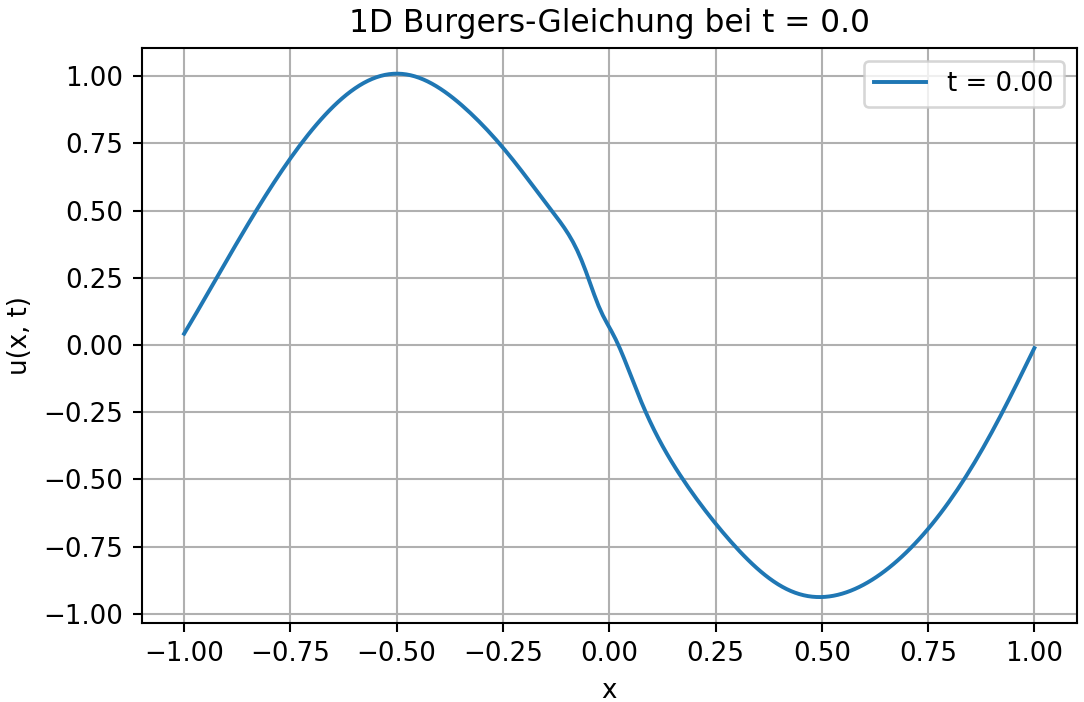
\includegraphics[width=0.48\textwidth]{papers/neuronal/images/burgers_solution_t0.png}\hfill
    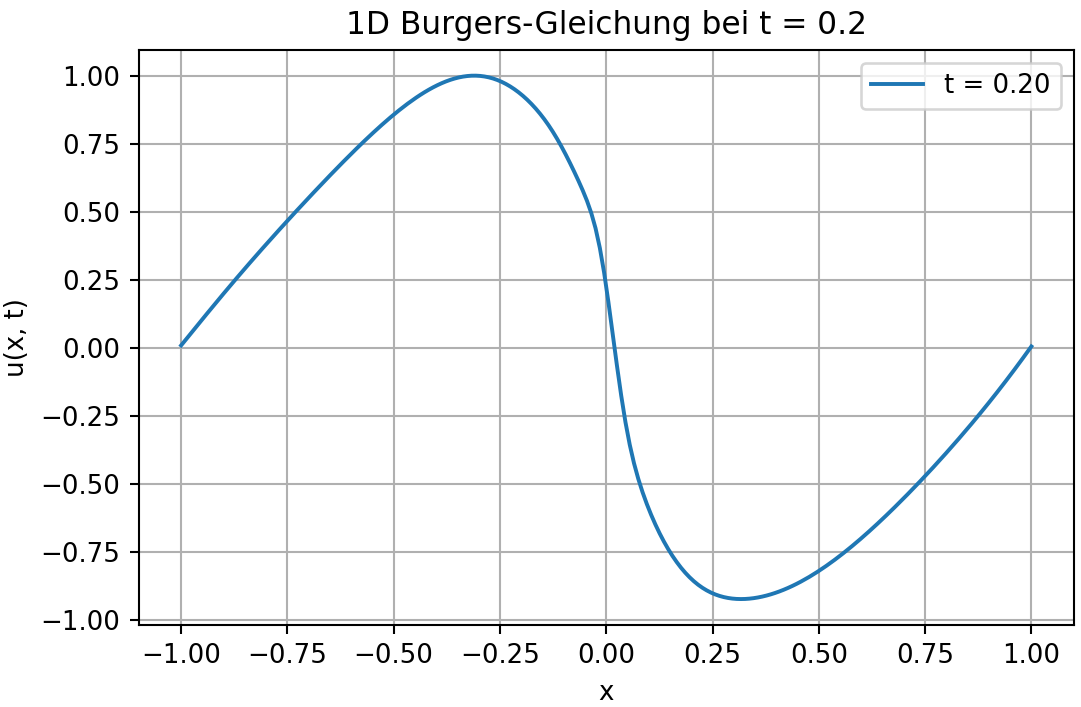
\includegraphics[width=0.48\textwidth]{papers/neuronal/images/burgers_solution_t02.png}
    \\[\smallskipamount]
    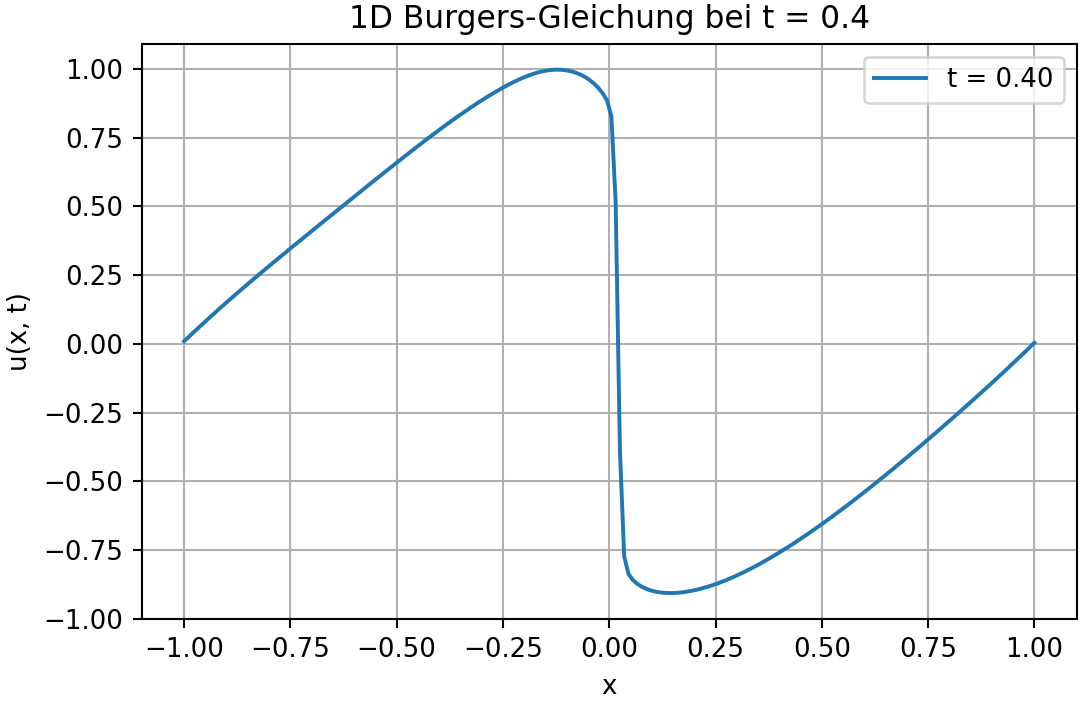
\includegraphics[width=0.48\textwidth]{papers/neuronal/images/burgers_solution_t04.png}\hfill
    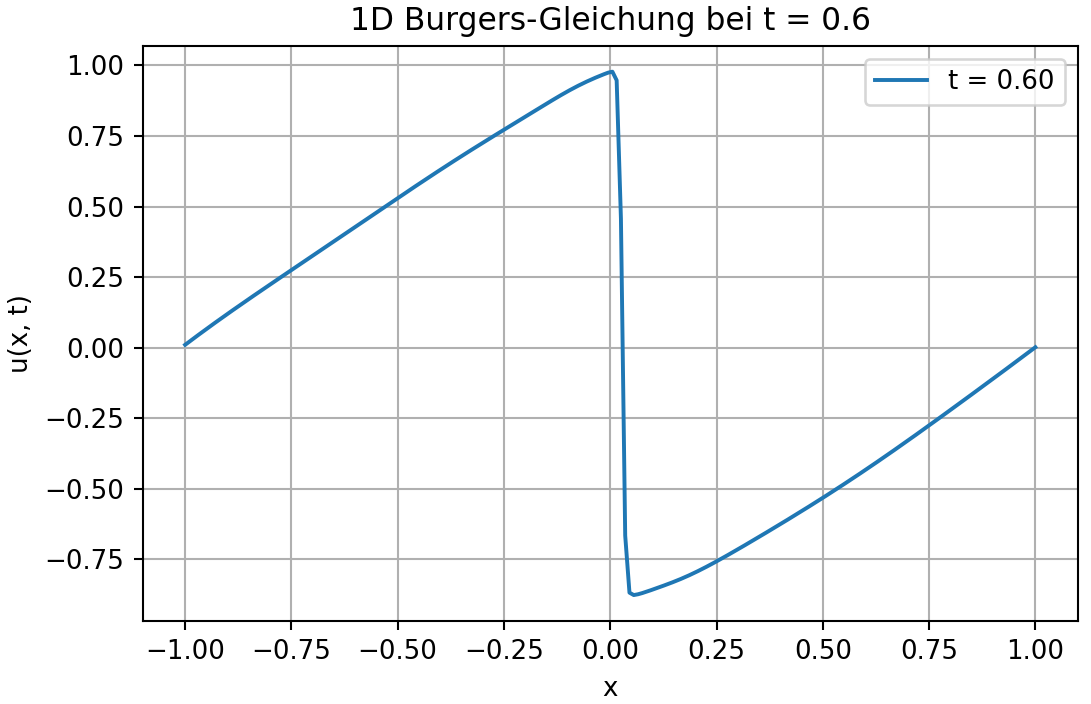
\includegraphics[width=0.48\textwidth]{papers/neuronal/images/burgers_solution_t06.png}
    \caption{Lösungs-Plot der Burgers-Gleichung zu verschiedenen Zeiten}\label{fig:loesung_burgers_fix_zeit}
\end{figure}
